\documentclass{article}

\usepackage{coursenotes}

\set{AuthorName}{TC Fraser}
\set{Email}{tcfraser@tcfraser.com}
\set{Website}{www.tcfraser.com}
\set{ClassName}{Electricity \& Magnetism 3}
\set{School}{University of Waterloo}
\set{CourseCode}{Phys 442}
\set{InstructorName}{Chris O'Donovan}
\set{Term}{Fall 2016}
\set{Version}{1.0}

\draftprofile[TC Fraser]{TC}{Purple}

\begin{document}

\titlePage

\tableOfContents

\disclaimer

\section{Coordinates and Symmetry}

A clever choice of coordinates systems typically makes solving a problem considerably easier. Mathematically, this is due to \textit{Noether's Theorem}. A typical three dimensional Lagrangian will have three dependent generalized coordinates $L = L \br{x,y,z} = L \br{s,\theta,\zeta} = \cdots$. However, if one can identify generalized coordinates $q$ that make the Lagrangian invariant $\pder{L}{q} = 0$, then the \textit{Euler-Lagrange} equations are considerably similar,
\[ \der{}{t}\br{\pder{L}{\dot{q}}} - \pder{L}{q} = 0 \implies \pder{L}{\dot{q}} = \textrm{const.} \implies L \propto \dot{q} \]
As such, the number of equations that remain to solved has been reduced.

\section{First Assignment?}

\newcommand{\coord}[4]{\coordinate (#1) at (#2,#3,#4);}
\newcommand{\cylindcoord}[4]{\coordinate (#1) at ({#2*cos(#3)},{#2*sin(#3)},{#4});}
\newcommand{\spherecoord}[4]{\coordinate (#1) at ({#2*cos(#3)*sin(#4)},{#2*sin(#3)*sin(#4)},{#2*cos(#4)});}

%polar coordinates of visibility
\pgfmathsetmacro\th{70}
\pgfmathsetmacro\az{110}
\tdplotsetmaincoords{\th}{\az}

\begin{center}

\begin{tikzpicture} [scale=1, tdplot_main_coords, axis/.style={->,black}]

    %parameters of the cone
    \pgfmathsetmacro\R{1.6} % Radius of cylinder
    \pgfmathsetmacro\H{3} % Height of cylinder
    \pgfmathsetmacro\aL{3.5} % Length of the axis

    \pgfmathsetmacro\rr{4}
    \pgfmathsetmacro\r{4}
    \pgfmathsetmacro\rphi{60}
    \pgfmathsetmacro\rh{4}
    \cylindcoord{r}{\rr}{\rphi}{\rh}
    \cylindcoord{rflat}{\rr}{\rphi}{0}
    \cylindcoord{rp}{\R}{-40}{1.4}
    \cylindcoord{radius}{\R}{-60}{0}
    \cylindcoord{hmark}{1.8}{-70}{0}
    \cylindcoord{hmarktop}{1.8}{-70}{\H}

    % Axis declaration
    \coordinate (O) at (0,0,0);
    \coordinate (x) at (1,0,0);
    \coordinate (y) at (0,1,0);
    \coordinate (z) at (0,0,1);
    \coordinate (X) at ($\aL*(x)$);
    \coordinate (Y) at ($\aL*(y)$);
    \coordinate (Z) at ($\aL*(z)$);

    %draw axes
    \draw[axis] (O)--(X) node[anchor=north]{$\hat{x}$};
    \draw[axis] (O)--(Y) node[anchor=north]{$\hat{y}$};
    \draw[axis] (O)--(Z) node[anchor=south]{$\hat{z}$};

    % % angles for transformed lines
    \pgfmathsetmacro\PhiOne{180+(\az)}
    \pgfmathsetmacro\PhiTwo{0+(\az)}

    % % coordinates for transformed surface lines
    \pgfmathsetmacro\sinPhiOne{{sin(\PhiOne)}}
    \pgfmathsetmacro\cosPhiOne{{cos(\PhiOne)}}
    \pgfmathsetmacro\sinPhiTwo{{sin(\PhiTwo)}}
    \pgfmathsetmacro\cosPhiTwo{{cos(\PhiTwo)}}

    % % draw basis circle
    \tdplotdrawarc[tdplot_main_coords]{(O)}{\R}{\PhiOne}{360+\PhiTwo}{}{}
    \tdplotdrawarc[tdplot_main_coords]{(O)++($\H*(z)$)}{\R}{0}{360}{}{}
    \tdplotdrawarc[tdplot_main_coords,dashed]{(O)}{\R}{\PhiTwo}{\PhiOne}{}{}

    \tdplotdrawarc[tdplot_main_coords,color=red]{(O)}{0.3}{0}{\rphi}{anchor=north}{$\phi$}

    % % displaying tranformed surface of the cone (rotated)
    \draw (\R*\cosPhiOne,\R*\sinPhiOne,\H) -- (\R*\cosPhiOne,\R*\sinPhiOne,0);
    \draw (\R*\cosPhiTwo,\R*\sinPhiTwo,\H) -- (\R*\cosPhiTwo,\R*\sinPhiTwo,0);

    \draw[thick,color=red, ->] (O) -- node[midway, below]{$\vr$} (r);
    \draw[thick,color=blue, ->] (O) -- node[midway, below]{$\vr'$} (rp);
    \draw[thick, ->] (rp) -- node[midway, below]{$\vec{\rcurs}$} (r);
    \draw[dashed,color=red, ->] (O) -- node[midway, below left]{$s\hat{s}$} (rflat);
    \draw[dashed,color=red, ->] (rflat) -- node[midway, right]{$\zeta\hat{\zeta}$} (r);
    \draw[->] (O) -- node[midway, below]{$R$} (radius);
    \draw[|<->|] (hmark) -- node[midway, left]{$h$} (hmarktop);

\end{tikzpicture}
\end{center}

\textbf{A1.1}: Use cylindrical coordinates with $\zeta$ along the axis of the cable,

\[ V\br{\zeta} = \f{1}{4 \pi \ep_0} \int_{\s{C}}\f{\dif \rho}{\rcurs} \]

Where $\ve{\rcurs} = \ve{r} - \ve{r}'$, $\ve{r}'$ is the source point and $\ve{r}$ is the field point. The entire cylinder is the set of all source points $\ve{r}'$ that are contained inside $\abs{\ve{r}'} \leq R$.
\[ \ve{r} = \zeta \hat{\zeta} \]
\[ \ve{r}' = s' \hat{s}' + \zeta' \hat{\zeta} \]

\[ V\br{\zeta} = \f{\rho}{4 \pi \ep_0} \int_{\s{C}}\f{\dif V}{\abs{\ve{r} - \ve{r}'}} \]

Where $ \dif V = s \dif s \dif \theta \dif \zeta$. One can then find the electric \textit{field} by doing $\ve{E} = - \vdel V = E_{\zeta} \hat{\zeta} = -\pder{V}{\zeta} \hat{\zeta}$

\textbf{A1.2}:

Between the two conductors, there will be a radial electric field $\ve{E} = E\br{s} \hat{s}$ and parallel magnetic field $\ve{B} = B\br{s} \hat{\zeta} $. Outside the two conductors, there will be no electric or magnetic field.

\[ E^{\parallel}\tsb{vac} = 0 \]
\[ E^{\perp}\tsb{vac} = \f{\si}{\ep_0} \]
\[ \vdel \cdot \ve{E} = \f{\rho}{\ep_0} \]

For part g), use Laplace's equation $\del^2 V = 0$. In cylindrical coordinates, Laplace's equation is,
\[ \del^2 V = \f{1}{s} \pder{}{s}\br{s \pder{V}{s}} = 0 \]
Cylindrical coordinates gives us the following symmetries $\pder{V}{\phi} = \pder{V}{\zeta} = 0$.
Solving this system gives the potential in terms of $s$: $V\br{s} = \cdots$. Then the electric field can then be obtained via $\vec{E} = - \vdel V$.

\textbf{A1.3}: Using cylindrical coordinates once again, the electric field is going to be radial outwards to the uniform charge density. For the uniform density cylinder, construct a Gaussian surface cylindrically around the cylinder. For the current density cylinder, the current density is the current per cross sectional area. Construct an Amperian loop,
\[ \oint_{\s{A}} \dif \vec{\ell} \cdot \vec{B} = \mu I\tsb{enc}  \]
Part e), finding the vector potential,
\[ A\br{\vr} = \f{\mu_0}{4\pi} \int_{\s{C}} \dif \tau' \f{\vec{J}\br{\vec{r}}}{\rcurs} \]
Evidently, $\hat{s}$ and $\hat{s}'$ are in \textit{different} directions.
Solving such an equation yields,
\[ A\br{s} = \f{\mu_0}{4 \pi} \int_{0}^{2\pi} \dif \phi' \int_{0}^{a} s' \dif s' \int_{-\inf}^{\inf} \dif \zeta' \f{J\br{s}}{\abs{s \hat{s} - s' \hat{s}' - \zeta' \hat\zeta}} \]
Recognize the structure of the potential integral,
\[ V\br{s} = \f{1}{4\pi \ep_0} \int_{\s{C}} \dif \tau' \f{\rho\br{r'}}{\rcurs} = \f{\rho_0}{4 \pi \ep_0} \int_{\s{C}} \f{\dif \tau'}{\rcurs}\]
Comparing to the vector potential, we have an equivalent integral (up to a constant).
\[ A\br{s} = \f{\mu_0 J_0}{4 \pi} \int_{\s{C}} \f{\dif \tau'}{\rcurs} \]
For question f), use the definition of $\vec{B}$ in terms of $\vec{A}$,
\[ \vec{B} = \vdel \times \vec{A} \]
Further, recall that if $\vec{E} = -\vdel V$, then by Stoke's theorem for some loop $\s{L}$,
\[ V = - \int_{\s{L}} \dif \vec{\ell} \cdot \vec{E} \]

\section{Conservation Laws}
Beginning with one of Maxwell's equations,
\[ \vdel \times \vec{B} = \mu_0 \vec{J} + \mu_0 \ep_0 \pder{\vec{E}}{t} \]
Taking the divergence of the above equation,
\[ \cancelto{0}{\vdel \cdot \br{\vdel \times \vec{B}}} = \mu_0 \vdel \cdot \vec{J} + \mu_0 \ep_0 \pder{}{t}\br{\vdel \cdot \vec{E}} \]
Luckily, the divergence of a curl is always $0$. Dividing by relevant constants we obtain the following conservation law,
\[ 0 = \vdel \cdot \vec{J} + \pder{\rho}{t} \eq \label{eq:conservation_charge}\]
This is a conservation of charge. It is a \textbf{local} conservation law because it holds for all points in space $\vec{r}$. Intuitively, is claims that the rate of charge of charge at a point is equal to the amount of current following in or out of the take point. \\

\textbf{A2.1}: Again using cylindrical coordinates $\vec{r} = s \hat{s} + \zeta \hat{\zeta}$. Let the current flow in such a way that the magnetic field points along the $\zeta$-axis. Let $\s{L}$ be an Amperian loop with one side at distance $\abs{\vec{r}} \to \inf$,
\[ \int_{\s{L}} \dif \vec{\ell} \cdot \vec{B} = \mu_0 I\tsb{enc} \]
The same equation can be reused to calculate the vector potential for a Gaussian surface $\s{S}$,
\[ \int_{\s{L}} \dif \vec{\ell} \cdot \vec{A} = \int_{\s{S}} \dif \vec{a} \cdot \vec{B} = \Phi \]
Where $\Phi$ is the magnetic flux through $\s{S}$. Furthermore, the energy required to set up a magnetic field is,
\[ W = \f{1}{2 \mu_0} \int_{\s{C}} \dif \tau B^2 = \f{1}{2} \int_{\s{C}} \dif \tau \vec{J} \cdot \vec{A} = \f{1}{2} L I^2 \]
Where $L$ is the self-inductance of the solenoid.

\section{Poynting's Theorem}
First we begin with two of Maxwell's equations,
\[ \vdel \times \vec{E} = - \pder{\ve B}{t} \eq \label{eq:poyn_max_1}\]
\[ \vdel \times \vec{B} = \mu_0 \vec{J} + \mu_0 \ep_0 \pder{\vec{E}}{t} \eq \label{eq:poyn_max_2}\]
Computing the inner product between \cref{eq:poyn_max_1} and $\vec{B}$, and the inner product between \cref{eq:poyn_max_2} and $\vec{E}$ and taking a difference,
\[ \vec{B} \cdot \br{\vdel \times \vec{E}} - \vec{E} \cdot \br{\vdel \times \vec{B}} = - \pder{}{t}\br{\f{\ep_0}{2} E^2 + \f{1}{2 \mu_0} B^2} = \mu_0 \vec{E} \cdot \vec{J}\]
Letting $\f{\ep_0}{2} E^2 + \f{1}{2 \mu_0} B^2$ be the \textbf{electromagnetic energy density} $u$, we have the following identity,
\[ \vdel\cdot\br{\vec{E} \times \vec{B}} = - \mu_0 \pder{u}{t} - \mu_0 \vec{E} \cdot \vec{J} \eq \label{eq:poyn_conservation_energy} \]
Physically \cref{eq:poyn_conservation_energy} corresponds to a conservation of energy. We refer to the term $\f{1}{\mu_0} \br{\vec{E} \times \vec{B}}$ as the Poynting vector $\vec{S}$ as it determines the direction of electromagnetic radiation. The Poynting vector $\vec{S}$ represents the power density.
\[ \vdel \cdot \vec{S} + \pder{u}{t} + \vec{E} \cdot \vec{J} = 0 \eq \label{eq:poyn_eq}\]
Much like \cref{eq:conservation_charge}, \cref{eq:poyn_eq} is a local conservation of \textit{energy}. The only algebraic difference is the term $\vec{E} \cdot \vec{J}$. If there is a flowing charge $\vec{J}$ through an electric field $\vec{E}$, then there is work done on the charge. By Gauss's theorem, the energy leaving through a surface $\s{S}$ per unit time is,
\[ \int_{\s{V}} \vdel \cdot \vec{S} \dif \tau =  \oint_{\s{S}} \dif \vec{a}\cdot \vec{S} \]
and the E-M energy in the volume $\s{V}$ is given by,
\[ \int_{\s{V}} \dif \tau u \]
Where again, $u$ is the electromagnetic energy density. If we integrate over \cref{eq:poyn_eq},
\[\int_{\s{V}} \dif \tau \br{\vdel \cdot \vec{S} +\pder{u}{t} + \vec{E} \cdot \vec{J}} = \oint_{\s{S}} \dif \vec{a}\cdot \vec{S} + \int_{\s{V}} \dif \tau \pder{u}{t} + \int_{\s{V}} \dif \tau \vec{E} \cdot \vec{J} \]
Each term in \cref{eq:poyn_eq} has it's purpose illuminated. The final term $\int_{\s{V}} \dif \tau \vec{E} \cdot \vec{J}$ corresponds to the work done on moving charges $\vec{J}$ in the volume $\s{V}$. In it important to note that there are no terms that corresponding to ``magnetic work''. \\

Consider the work done to move a charge $q$ a displacement $\dif \vec{\ell}$ by E-M forces,
\begin{align*}
\dif W &= \dif \vec{\ell} \cdot \vec{F} \\
&= \dif \vec{\ell} \cdot q \br{\vec{E} + \vec{v} \times \vec{B}}\\
&= \vec{v} \dif t \cdot q \br{\vec{E} + \vec{v} \times \vec{B}}\\
&= q \dif t \br{\vec{v} \cdot \vec{E}} + q \dif t \underbrace{\br{\vec{v} \cdot \bc{\vec{v} \times \vec{B}}}}_{= 0} \\
&= q \dif t \br{\vec{v} \cdot \vec{E}}
\end{align*}
So for a continuous charge distribution we have that $\dif q = \rho \dif \tau$ and $\rho \vec{v} = \vec{J}$. Which means that the rate of work done on the charge $\rho$ in the volume $\s{V}$ (i.e. creating the current density $\vec{J}$) is,
\[ \dot{W} = \int_{\s{V}} \dif \tau \vec{E} \cdot \vec{J} \]
We can interpret this as the work done per unit time rearranging the charge in $\s{V}$. One again \cref{eq:poyn_eq} is given by
\[ \vdel \cdot \vec{S} + \pder{u}{t} + \vec{E} \cdot \vec{J} = 0 \]
With the following interpretations,
\begin{itemize}
    \item $\vdel \cdot \vec{S}$: amount of radiation energy leaving the point $\vr$
    \item $\pder{u}{t}$: increase in E-M energy at the point $\vr$
    \item $\vec{E} \cdot \vec{J}$: the amount of work done on charges at the point $\vr$
\end{itemize}

% \begin{tikzpicture}
%     \draw[thin, dashed] (0,0) circle (2);
%     \draw[fill] (0,0) circle (0.1);
% \end{tikzpicture}

As an illustrative example, consider a parallel plate capacitor with an electric field $\vec{E}$ between them.
\begin{center}
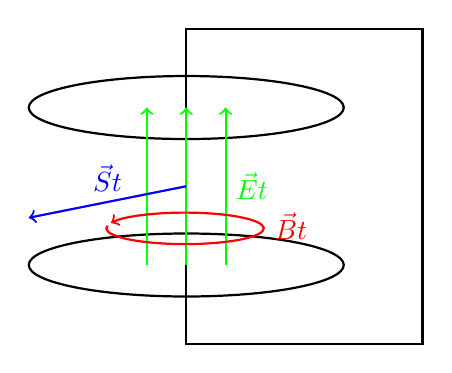
\begin{tikzpicture}
    \coordinate (top) at (0,1);
    \coordinate (bot) at (0,-1);
    \draw[thick] (top) ellipse (2 and 0.4);
    \draw[thick] (bot) ellipse (2 and 0.4);
    \draw[thick] (top) -- (0, 2) -- (3, 2) -- (3, -2) -- (0, -2) -- (bot);
    \draw[thick, green] (top) edge[<-] (bot);
    \draw[thick, green] (0.5, 1) edge[<-] node[midway, right]{$\vec{E}\br{t}$} (0.5, -1);
    \draw[thick, green] (-0.5, 1) edge[<-] (-0.5, -1);
    \draw[thick, blue] (0, 0) edge[->] node[midway, above]{$\vec{S}\br{t}$} (-2, -0.4);
    \draw[->, thick, red] (-1,-0.5) arc [start angle=-190, end angle=160, x radius=1, y radius=0.2];
    \draw[red] (1, -0.5) node[right]{$\vec{B}\br{t}$};
\end{tikzpicture}
\end{center}
We ave that the magnetic field points in the $\hat{\phi}$ direction, $\vec{B} = V \hat{\phi}$. The electric field $\vec{E} = E \hat{\zeta}$, and Poynting vector are $\vec{S} = S \hat{s}$. We have that the radiation through the surface $\s{S}$,
\[ \int_{\s{S}} \dif \vec{a} \cdot \vec{S} = - \br{2 \pi a h} S \]
Therefore $\pder{U}{t} = - \br{2 \pi a h} S$ corresponding to the amount of energy flowing out of the capacitor and therefore,
\[ U = \intl_{0}^{\inf} \dif t \br{- 2 \pi a h S} = \f12 C V^2 \]

\textbf{Ex 8.1}:
\begin{center}
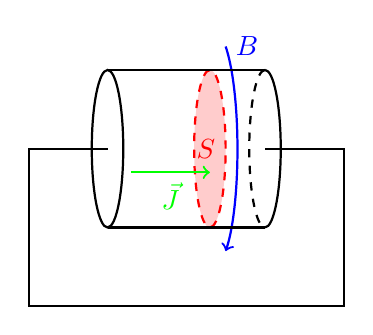
\begin{tikzpicture}
    \pgfmathsetmacro\R{1} % Radius of cylinder
    \coordinate (top) at (\R,0);
    \coordinate (bot) at (-\R,0);
    \coordinate (topshift) at (\R,\R);
    % \draw[thick] (top) ellipse (0.2 and 1);
    \draw[thick] (bot) ellipse (0.2 and 1);
    \draw[thick, dashed] (\R, \R) arc [start angle=90, end angle=270, x radius=0.2, y radius=1];
    \draw[thick] (\R, -\R) arc [start angle=-90, end angle=90, x radius=0.2, y radius=1];
    \draw[thick, blue, <-] (0.5, -1.3) arc [start angle=-60, end angle=60, x radius=0.3, y radius=1.5];
    \draw[thick, blue] (0.5, 1.3) node[right]{$\ve{B}$};
    \draw[thick, dashed, red, fill, fill opacity=0.2] (0.5, 0) arc [start angle=0, end angle=360, x radius=0.2, y radius=1] node[left, fill opacity=1.0]{$\s{S}$};
    \draw[thick] (\R, \R) -- (-\R, \R);
    \draw[thick] (\R, -\R) -- (-\R, -\R);
    \draw[thick] (top) -- (2, 0) -- (2, -2) -- (-2, -2) -- (-2, 0) -- (bot);

    \draw[thick, green] (-0.7, -0.3) edge[->] node[below]{$\vec{J}$} (0.3, -0.3);
\end{tikzpicture}
\end{center}
Inside the conductor the electric field moves parallel to its axis $\vec{E} = \f{V_0}{\ell} \hat{\zeta}$. The magnetic field is then given by,
\[ \vdel \times \vec{B} = \mu_0 \ep_0 \pder{E}{t} + \mu_0 \vec{J} \]
Integration over the surface $\s{S}$,
\[ \int_{\s{S}} \dif \vec{a} \cdot \br{\vdel \times \vec{B}} = \mu_0 \int_{\s{S}} \dif \vec{a} \cdot \vec{J} = \mu_0 I\tsb{enc} \]
Therefore computing this integral $\int \dif \vec{\ell} \cdot \vec{B}$ yields,
\[ \vec{B} = \f{\mu_0I}{2\pi a}\hat{\phi} \]
Moreover, the Poynting vector is given by,
\begin{align*}
\vec{S} &= \f{1}{\mu_0} \vec{E}\times \vec{B} \\
&= \f{1}{\mu_0} \f{V_0}{\ell} \hat{\zeta} \times \f{\mu_0 I}{2 \pi a} \hat{\phi} \\
&= -\f{V_0 I}{2\pi a \ell}\hat{s}
\end{align*}
Therefore the radiation flux,
\[ \int_{\s{S}} \dif \vec{a} \cdot \vec{S} = -\f{V_0 I}{2 \pi a \ell} \int_{\s{S}} \dif a = - V_0 I \]
Which is exactly the amount of Joule heating for a current $I$ though a wire with voltage $V_0$ across it. Using $V = I R$,
\[ \int_{\s{S}} \dif \vec{a} \cdot \vec{S} = -I^2 R \]
\textbf{Ex 8.2 (Griffiths Problem 8.13):}
A long thin solenoid of radius $a$ has a time dependent current $I_{s}\br{t}$ flowing around it. Encircling the solenoid is a ring of radius $b$ with current $I_{r}\br{t}$ ($b \gg a$) passing through it. The ring has resistance $R$. There is an induced electro-motive-force in the ring due to the solenoid,
\[ \s{E} = - \dot{\Phi}_S = - \pder{}{t}\br{\pi a^2 B_S} \]
Where $B_s = \mu_0 n I_s$. The EMF $\s{E}$ must also equal $\s{E} = I_r R$. Therefore,
\[ I_r = - \f{1}{R}\br{\mu_0 \pi a^2 n}\dot{I}_S \]
In order to calculate the electric and magnetic fields just outside solenoid, recognize that $\ve B_s = B_s\br{t} \hat{z}$ point along the axis of the solenoid. Similarly recognize that $\ve E = E \hat{\phi}$. Therefore the Poynting vector is given by,
\[ \ve S = \f{1}{\mu_0} \ve E \times \ve B_s = \f{1}{\mu_0} E B_{s} \hat{s} = ? \]
We first need to calculate $\ve E$ and $\ve B_s$. The magnetic field is known to be $\ve B = \mu_0 n I_s \hat{z}$ on axis and $\vdel \times \ve E = - \pder{\ve B}{t}$,
\[ \int \dif \ve a \cdot \vdel \times \ve E = - \der{}{t} \int \dif \ve a \cdot \ve B \]
\[ \int \dif \ve \ell \cdot \ve E = - \dot \Phi = 2 \pi a E \]
Which gives,
\[ \ve E = \f{\dot \Phi}{2\pi a}\hat{\phi} \]
The magnetic field off axis and outside the solenoid due to the ring is given by,
\[ \dif \ve B_r \br{s} = \f{\mu_0 I}{4 \pi} \f{\dif \ve \ell \times \ve \rcurs}{\rcurs^2} \]
Where $\ve \rcurs = \ve r - \ve r'$ and we take $\ve r ' = b \hat s '$ and $\ve r = z \hat z$.
\[ \ve \rcurs = z \hat z - b \hat s' \]
We will take the infinitesimal loop to be $\dif \ve \ell = b\dif \phi'\hat \phi'$.
\begin{align*}
\dif \ve \ell \times \ve \rcurs &= \br{b \hat \phi' \dif \hat \phi'}\times\br{z\hat z - b \hat s '} \\
&= a z \dif \phi' \hat s' + b^2 \dif \phi' \hat z
\end{align*}
We integrating around the loop $\s{L}$, all of the contributions in the $\hat{s}'$ directions will cancel out.
\[ \int_{\s{L}} \dif \ve \ell \times \ve \rcurs = \cdots \]
Thus,
\begin{align*}
\ve B_r &= \f{\mu_0 I_r}{4\pi} \int \f{b^2 \dif \phi' \hat z}{\br{z^2 + b^2}^{3/2}} \\
&= \f{\mu_0 I_r b^2 2 \pi \hat z}{4\pi \br{z^2 + b^2}^{3/2}} \\
&= \f{\mu_0 b^2}{2\br{z^2 + b^2}^{3/2}}I_r\hat z
\end{align*}
Therefore the Poynting vector points radial outward,
\begin{align*}
\ve S &= \f{1}{\mu_0}\ve E_r \times \ve B_r \\
&= \f{1}{\mu_0}\br{\f{\pi a^2 \mu_0 n \dot I_s}{2 \pi a} \hat \phi} \times \br{\f{\mu_0 b^2}{2\br{z^2 + b^2}^{3/2}}I_r\hat z} \\
&= \f{\mu_0}{4} a n \dot I_s \f{b^2}{\br{z^2 + b^2}^{3/2}} I_r \hat{s}
\end{align*}
Now that the Poynting vector is known, one can calculate the power radiated from the system.
\begin{align*}
P &= \int \dif \ve a \cdot \ve S \\
&= \f{\mu_0}{4} a n \dot I_s I_r b^2 \int \dif z a \dif \phi \hat s \cdot \f{1}{\br{z^2 + b^2}^{3/2}} \hat{s} \\
&= \f{\mu_0}{4} a n \dot I_s I_r b^2 \br{2 \pi a} \int \dif z \f{1}{\br{z^2 + b^2}^{3/2}} \\
&= \f{\mu_0}{4} a n \dot I_s I_r b^2 \br{2 \pi a} \f{2}{b^2} \note{Integral Table} \\
&= \mu_0 \pi a^2 n \dot I_s I_r
\end{align*}
But we know that $\mu_0 \pi a^2 n \dot I_s = - I_r R$. Therefore $P = - I_r^2 R$ as expected.\\
\textbf{A2.2:}\\
a,b) Answers in Griffiths. \\
c) Consider parallel metal strips with height $h$ and width $w$ where $h \ll w$. A current flows down one plate and up the other. The system will act as a capacitor. The magnetic field outside will be zero and non-negative inside. \\
d) Griffiths 8.1 \\
\textbf{A2.3:}\\
Positive and negative charge build up on the surfaces between the capacitor. Of course, there will be a time varying current $I\br{t}$, electric field $\ve E \br{t}$ and magnetic field $\ve B \br{t}$.
\section{Stress Energy Tensor}

Last week we looked at conservation laws and we found,
\[ \vdel \cdot \ve J + \pder{\rho}{t} = 0 \note{(charge)} \]
and,
\[ \vdel \cdot \ve S + \pder{u}{t} + \ve J \cdot \ve E = 0 \note{(energy)} \]
This week we will continue with momentum and angular momentum and then we will examine the Maxwell stress tensor; the field equivalent for force in Newton's second law. But first we will look at momentum.
\subsection{Momentum}
Consider two charges $+q_1$ and $-q_2$ with velocities $\ve v_1$ and $\ve v_2$. The electric field at point $2$ due to charge $1$ will be denoted $\ve E_1$. Analogously for $\ve B_1$. The net force acting on charge $q_2$ is then,
\[ \ve F_{2;E} = q_2 \ve E_1 \qquad \ve F_{2;B} = q_2 \ve v_2 \times \ve B_1 \]
\[ \ve F_{1;E} = q_1 \ve E_2 \qquad \ve F_{1;B} = q_1 \ve v_1 \times \ve B_2 \]
One will notice that $\ve F_{1;B}$ and $\ve F_{2;B}$ are not equal and opposite forces like $\ve F_{1;E}$ and $\ve F_{2;E}$ are. What does this say about Newton's third law?
\[ \sum \dve p_i = \sum \ve F\tsb{net} \]
We forgot about the fact that the electric and magnetic fields carry not only energy (via $\ve S$) but momentum as well. Recall that for photons,
\[ E = h f = \hbar \w  \]
\[ p = \f{h}{\la} = \hbar k \]
Therefore we have that,
\[ E = pc \]
Therefore knowing the energy density of the field gives you then momentum density of the field. The momentum density will be denoted $\ve g$.
\[ \ve g = \f{1}{c^2} \ve S = \mu_0 \ep_0 \ve S = \f{1}{4 \pi c} \ve E \times \ve B \]
The force per unit volume $\ve f = \De \ve F / \De \tau$ acting on a particle is given by the Lorrentz force.
\[ \ve f = \rho \ve E + \ve J \times \ve B\]
Which when expanded out is,
\[ \ve f = \ep_0 \br{\vdel \cdot \ve E} \ve E + \br{\f{1}{\mu_0} \vdel \times \ve B - \ep_0 \pder{\ve E}{t}} \times \ve B \]
\todo[TC]{Inject hand out}
Which after some algebra yields,
\[ \ve f = \ep_0 \br{\br{\vdel \cdot \ve E} \ve E + \br{\ve E \cdot \vdel} \ve E} + \f{1}{\mu_0} \br{\br{\vdel \cdot \ve B} \ve B + \br{\ve B \cdot \vdel} \ve B} - \vdel \br{\f{\ep_0}{2} E^2 + \f{1}{2 \mu_0} B^2} - \mu_0 \ep_0 \pder{\ve S}{t} \eq \label{eq:messy}\]
We now introduce \term{Maxwell's stress energy tensor} $T$ with components,
\[ T_{ij} = \ep_0 \br{E_i E_j - \f{1}{2} \de_{ij} E^2} + \f{1}{\mu_0} \br{B_i B_j - \f{1}{2} \de_{ij} B^2} \]
Where $\ve E = \sum_{i} E_i \hat{e}_i$ and $\ve B = \sum_{i} B_i \hat{e}_i$. We now have that \cref{eq:messy} gives,
\[ \ve f = \vdel \cdot T - \ep_0 \mu_0 \pder{\ve S}{t} \]
As defined $\ve F = \int_{\s{V}} \dif \tau \ve f$ is the net mechanical force acting on the matter in a volume $\s{V}$. Therefore,
\begin{align*}
\der{}{t} \ve p\tsb{mech} &= \int_{\s{V}} \dif \tau \ve f \\
&= \int_{\s{V}} \dif \tau \br{\vdel \cdot T - \ep_0 \mu_0 \pder{S}{t}} \\
&= \oint_{\s{S}} \dif a \cdot T - \der{}{t} \int_{\s{V}} \dif \tau \ep_0 \mu_0 \ve S
\end{align*}
We usually define the second term here to be the momentum contained in the electromagnetic field,
\[ \ve p\tsb{em} = \int_{\s{V}} \dif \tau \ep_0 \mu_0 \ve S \]
Therefore the conservation of momentum is,
\[ \der{}{t} \br{\ve p\tsb{mech} + \ve p\tsb{em}} = \oint_{\s{S}} \dif a \cdot T \]
\subsection{Cauchy Stress Tensor}
The \term{Cauchy stress tensor} is a representation of the total forces acting on a chunk $\s{V}$ of a material due to the neighboring pieces $\s{N}\br{\s{V}}$. Each neighboring chunk $n \br{\s{V}}$ can exert parallel or shear forces on $\s{V}$. This defines a matrix on force components on each face of $\s{V}$. Let $\ve f = \si \cdot \dif \ve a$ where $\ve{\si}$ is a rank 2 (3d) tensor. We call $\si$ the Cauchy stress tensor such that,
\[ \ve f = \si \cdot \dif \ve a \]


\end{document}
